\section{Deployment}
In questa sezione verranno trattate le scelte in materia di deployment dell'architettura, discuteremo le scelte effettuate per i servizi Azure utilizzati, la configurazione di tali servizi e l'automazione del processo di deployment, così come le soluzioni e strategie adottate per garantire scalabilità e affidabilità dell'applicazione.

\subsection{Componenti}
Per riferimento si riportano di seguito i componenti principali che costituiscono l'applicazione.
\begin{itemize}
    \item Middleware NBA Api
    \item Middleware Bet Api
    \item Frontend Applicazione Web
    \item Modello Machine Learning
\end{itemize}

Abbiamo preso la decisione di creare dei middleware per l'interazione con le api delle quote e delle statistiche NBA per creare una interfaccia che permette alla applicazione di non essere a conoscenza del funzionamento delle API sottostanti che forniscono i dati, questo approccio permetterà inoltre in futuro di modificare le API sottostanti per migliorare le prestazioni dell'applicazione.

L'applicazione deve essere in grado di adattarsi ad aumenti inaspettati del carico di richieste, per questo è stato necessario utilizzare servizi che supportassero funzionalità di scalabilità automatiche sia all'aumento del carico, sia alla sua diminuzione per mantenere il più possibile contenuti i costi del servizio.

Per la distribuzione dei due middleware abbiamo deciso di utilizzare container OCI in quanto sono lo strumento più adatto a effettuare il deployment di una architettura a microservizi.

\subsection{Servizi Azure}

Microsoft Azure offre una vasta gamma di servizi per qualsiasi tipo di deployment, la scelta del giusto servizio per un certo componente è cruciale per bilanciare costi di operazione del componente e massimizzare l'efficienza e automazione del processo di deployment minimizzando le interruzioni del servizio.

\subsubsection{Container}
Microsoft Azure offre varie opzioni per il deployment di componenti basati su container OCI, da cluster Kubernetes parzialmente gestiti a ambiente completamente gestiti:
\begin{itemize}
    \item Azure Container Instances (ACI)
    \item Azure Container Apps (ACA)
    \item Azure Kubernetes Services (AKS)
    \item Azure App Service (AAS)
\end{itemize}

Questi servizi hanno diversi livelli di complessità delle opzioni di configurazione, in particolare AKS è il servizio che offre la maggiore granularità nelle opzioni di gestione dei cluster di container: si tratta di una istanza di Kubernetes gestita da Azure che fornisce una piattaforma di orchestrazione completa adatta a deployment molto complessi.

Durante la valutazione delle opzioni abbiamo escluso il servizio AAS in quanto si tratta di un servizio non nativamente improntato a deployment di applicazioni sotto forma di container, non offre infatti le opzioni di gestione della scalabilità offerte da altri servizi concepito per container.

Mentre ACI offre una esperienza di deployment molto semplificata non da la possibilità di creare regole di scaling e replicazione personalizzate, ogni aspetto del deployment è gestito da Azure; ACA si pone a metà strada tra la semplicità di ACI e la complessità di AKS in quanto nasconde dettagli di gestione del cluster Kubernetes ma permette comunque di specificare regole e limiti di scaling con abbastanza granularità.

Abbiamo infine deciso di utilizzare Azure Container Apps per il deployment dei due microservizi.

Abbiamo distribuito i componenti middleware in un unico Azure Container App Environment, il componente che orchestra le ACA mantenendo aggiornamenti OS, procedure di recupero post-failure e bilanciamento delle risorse tra componenti, questo servizio gestisce inoltre la creazione e configurazione del virtual network che si pone a protezione delle ACA istanziate.

\subsubsection{Web Application}
Per effettuare il deployment dell'applicazione web abbiamo ristretto l'offerta di Azure a due servizi:
\begin{itemize}
    \item Azure Static Web App (SWA)
    \item Azure App Service (AAS)
\end{itemize}

Come in precedenza il servizio AAS risulta non adatto agli scopi dell'applicazione in quanto l'applicazione necessita solo di un frontend che comunica con i due microservizi, abbiamo quindi deciso di utilizzare il servizio SWA, un servizio che offre la possibilità di distribuire una webapp statica con gestione automatica di un CDN globale per garantire una distribuzione del contenuto veloce e affidabile.

Questo servizio offre anche la possibilità di associare un backend sotto forma di ACA o Azure Functions: in futuro sarà possibile aggiungere un nuovo microservizio che gestisca il backend dell'applicazione, implementando funzionalità come la creazione account utente.

\subsubsection{Modello Machine Learning}
Per rendere il modello accessibile al componente che ne deve mostrare i risultati abbiamo valutato diverse opzioni per creare appositi endpoint per richiedere una inferenza al modello.

La prima opzione che abbiamo considerato è stata creare un container apposito e utilizzare una ACA per rendere gli endpoint accessibili al frontend dell'applicazione, per quanto questa possa essere una soluzione appropriata in quanto avrebbe reso più uniforme l'architettura che fa già largamente uso di ACA, Azure offre una soluzione migliore apposita per modelli di machine learning.

Azure Machine Learning Workspace mette a disposizione un ambiente completamente fornito per ogni step della creazione e gestione di un modello di machine learning.

Le funzionalità principali che sono risultate utili sono le seguenti:
\begin{itemize}
    \item ambienti di sviluppo gestiti e configurabili
    \item categorizzazione e versioning dei modelli creati
    \item authoring di modelli tramite jupyter notebooks e strumenti di alto livello a componenti
    \item riusabilità dei componenti
    \item gestione automatica della cache di inferenze passate
    \item valutazione delle performance del modello tramite strumenti di analisi
\end{itemize}

Questo workspace permette inoltre di effettuare deployment dei modelli creati e di generare appositi endpoint HTTP per richiedere l'inferenza su una istanza del feature vector in modo sicuro, autenticando le richieste tramite chiavi api.

Durante il deployment del modello abbiamo riscontrato problematiche con la gestione delle politiche CORS: il sistema di deployment integrato non supporta la modifica delle politiche CORS per abilitare l'accesso da parte di una applicaizione web. Per risolvere questo problema abbiamo integrato questo endpoint in un endpoint presente nel Middleware NBA Api.

\subsubsection{Servizi di supporto}
I servizi appena descritti includono i componenti principali dell'applicazione, abbiamo però utilizzato diversi altri servizi Azure di supporto.

\paragraph{Gestione segreti} 
Una necessità immediatamente evidente durante lo sviluppo è stata quella di avere a disposizione un sistema centralizzato dove archiviare in modo sicuro vari segreti come chiavi api e certificati. Si presta a questo scopo il servizio Azure Key Vault che offre la possibilità di immagazzinare segreti gestendone il versionamento di questi ultimi.

Un'altra funzionalità che Key Vault offre è la possibilità di impostare la rotazione automatica di certificati crittografici, sfruttata dal sistema per rinnovare automaticamente i certificati legati al dominio personalizzato usato per raggiungere l'applicazione.

\paragraph{Gestione Immagini OCI}
Il sistema sfrutta diverse immagini OCI e deve essere in grado di gestirne il versionamento mantenendole private.

A questo scopo abbiamo sfruttato due istanze di Azure Container Registry, un servizio che offre la possibilità di immagazzinare definizioni di immagini con gestione delle versioni tramite tag, è inoltre meglio integrato con gli altri servizi di Azure di altri container registry.

Le credenziali per l'accesso all'istanza ACR principale, ovvero quella che contiene le immagini dei middleware, sono gestite tramite Azure Key Vault; la seconda istanza, dedicata alle immagini degli ambienti di sviluppo del Machine Learning Workspace, è completamente gestita dal Workspace stesso.

\paragraph{Gestione DNS}
Allo scopo di associare domini personalizzati ai servizi, in particolare alla applicazione web, abbiamo creato una Azure DNS Zone, risorsa che assume il compito di gestire la propagazione dei record DNS del dominio utilizzato.

Abbiamo fatto la scelta di trasferire il controllo dei DNS ad Azure per automatizzare il processo di provisioning dei certificati: questo processo necessita della creazione di record DNS temporanei per autenticare la creazione del certificato, dato che Azure è in controllo dei record può generare e verificare i certificati senza intervento.

\paragraph{Gestione Log}
Per la gestione dei log generati dai vari componenti dell'infrastruttura abbiamo fatto uso del servizio Azure Log Analitycs Workspace che offre una raccolta dei log centralizzata e mette a disposizione un linguaggio di query e altri strumenti per effettuare analisi sulle informazioni raccolte dai servizi.

\paragraph{Document Database}
Come supporto aggiuntivo alla cache delle richieste effettuate ai middleware, oltre ad alcuni accorgimenti effettuati nello sviluppo dei due componenti, abbiamo sfruttato un database a documenti per salvare i risultati di alcune richieste molto frequenti e che non necessitano di aggiornamenti frequenti.

\subsection{Provisioning Infrastruttura}
Data la vasta gamma di risorse Azure da gestire abbiamo deciso di utilizzare un sistema di provisioning automatizzato, a questo scopo abbiamo scelto lo strumento di Infrastructure as Code Terraform.

Tramite HCL, il linguaggio di configurazione di Terraform, è possibile definire l'infrastruttura da creare tramite appositi blocchi risorsa: ognuno di questi blocchi rappresenta una risorsa da generare e specifica tutti i parametri da configurare, come ad esempio immagine, regole di scalabilità e segreti per le ACA.

Tramite il comando \texttt{terraform apply} è possibile generare un piano di esecuzione ed eseguirlo: il risultato è la creazione delle risorse sull'abbonamento Azure specificato. Utilizzando il comando \texttt{terraform destroy} si da il via alla rimozione delle risorse specificate.

La rimozione di alcune risorse talvolta può incorrere in tempi molto lunghi, soprattutto se è necessario creare e distruggere spesso l'architettura, per questo motivo abbiamo specificato alcuni componenti Azure come datasource, questo tipo di risorse rappresenta un componente sulla piattaforma cloud del quale è solo necessario prelevare gli attributi: alla distruzione non verranno intaccate queste risorse. Esempi di queste risorse sono gli Azure Container Registry, l'Azure Key Vault e l'Azure Container App Environment che necessitano di essere sempre disponibili nell'infrastruttura.

Abbiamo incontrato varie problematiche con l'utilizzo di Terraform, giustificabile dal fatto che le risorse Azure subiscono modifiche alla tipologia di parametri di configurazione con frequenza abbastanza alta, soprattutto quei parametri legati a funzionalità in preview.

Un esempio di queste problematiche è relativa alla generazione di certificati per domini personalizzati per le Container App.

Un bug nella gestione dello stato Terraform del ciclo di vita dello stato di provisioning dei certificati impedisce la creazione di un certificato gestito da Azure e il suo provisioning senza intervento manuale dal portale Azure. A questo scopo abbiamo creato appositi script che sfruttano in modo programmatico (e non dichiarativo) Az CLI per sopperire alle mancanze dei moduli azure.

Di seguito si riporta come esempio lo script utilizzato per creare e effettuare il provisioning di un certificato TLS gestito da Azure, lo script viene usato in tandem con una \texttt{null\_resource} per includere l'operazione nello stato di Terraform.

\begin{minted}[bgcolor=lightgray,framesep=2mm,baselinestretch=1.2,fontsize=\footnotesize]{bash}
DOES_CUSTOM_DOMAIN_EXIST=$(
  az containerapp hostname list \
    -n $CONTAINER_APP_NAME \
    -g $RESOURCE_GROUP \
    --query "[?name=='$CUSTOM_DOMAIN'].name" \
    --output tsv
)
if [ -z "${DOES_CUSTOM_DOMAIN_EXIST}" ]; then
  echo "adding custom hostname to container app first since it does not exist yet"
  az containerapp hostname add \
    -n $CONTAINER_APP_NAME \
    -g $RESOURCE_GROUP \
    --hostname $CUSTOM_DOMAIN \
    --output none
fi

MANAGED_CERTIFICATE_ID=$(
  az containerapp env certificate list \
    -g $RESOURCE_GROUP \
    -n $CONTAINER_APP_ENV_NAME \
    --managed-certificates-only \
    --query "[?properties.subjectName=='$CUSTOM_DOMAIN'].id" \
    --output tsv
)
if [ -z "${MANAGED_CERTIFICATE_ID}" ]; then
  MANAGED_CERTIFICATE_ID=$(
    az containerapp env certificate create \
      -g $RESOURCE_GROUP \
      -n $CONTAINER_APP_ENV_NAME \
      --hostname $CUSTOM_DOMAIN \
      --validation-method CNAME \
      --query "id" \
      --output tsv
  )
  echo "created cert for '$CUSTOM_DOMAIN'. waiting for it to provision now..."

  tries=0
  until [ "$tries" -ge 20 ]; do
    STATE=$(
      az containerapp env certificate list \
        -g $RESOURCE_GROUP \
        -n $CONTAINER_APP_ENV_NAME \
        --managed-certificates-only \
        --query "[?properties.subjectName=='$CUSTOM_DOMAIN'].properties.provisioningState" \
        --output tsv
    )
    echo "checking cert status... $STATE"
    if [[ $STATE == "Succeeded" ]] ; then
      echo "certificate is ready, provisioning state Succeeded"
      break
    else
      tries=$((tries + 1))
    fi

    sleep 15
  done
  if [ "$tries" -ge 20 ]; then
    die "waited for 5 minutes, checked the certificate status 20 times and its not done.
    check azure portal..."
  fi
else
  echo "found existing cert in the env. proceeding to use that"
fi

# check if the cert has already been bound
# if not, bind it then
IS_CERT_ALREADY_BOUND=$(
  az containerapp hostname list \
    -n $CONTAINER_APP_NAME \
    -g $RESOURCE_GROUP \
    --query "[?name=='$CUSTOM_DOMAIN'].bindingType" \
    --output tsv
)
if [ $IS_CERT_ALREADY_BOUND = "SniEnabled" ]; then
  echo "cert is already bound, exiting..."
else
  # try bind the cert to the container app
  echo "cert successfully provisioned. binding the cert id to the hostname"
  az containerapp hostname bind \
    -g $RESOURCE_GROUP \
    -n $CONTAINER_APP_NAME \
    --hostname $CUSTOM_DOMAIN \
    --environment $CONTAINER_APP_ENV_NAME \
    --certificate $MANAGED_CERTIFICATE_ID \
    --validation-method CNAME \
    --output none
  echo "finished binding. the domain is now secured and ready to use"
\end{minted}

\subsection{Continuous Integration}
Allo scopo di velocizzare il deployment delle nuove versioni dei componenti rilasciate dagli sviluppatori, abbiamo creato workflow automatizzati per la generazione delle nuove immagini e il rilascio sulle istanze di Container App e Static Web App.

\subsubsection{Workflow bet-api}
Dato che Bet API è stata progettata usando Java abbiamo scelto Gradle come build system, implementando delle task personalizzate mirate a generare un Dockerfile, creare l'immagine e pubblicarla su Azure Container Registry.

Il workflow, rilasciato come Github Action, necessita di accedere ai dati delle credenziali per il registro: queste informazioni sono salvate come Github Secrets; questa soluzione, utilizzata anche nel workflow per NBA Api, si è resa necessaria a causa dell'impossibilità di configurare identità tramite Azure.

A causa di queste limitazioni sulla gestione dell'autenticazione non siamo stati in grado di aggiungere al workflow uno step per creare una nuova revisione basata sulla nuova immagine, questa operazione viene effettuata manualmente.

Di seguito si riporta un estratto delle task che generano l'immagine insieme al workflow Github Actions.

\begin{minted}[bgcolor=lightgray,framesep=2mm,baselinestretch=1.2,fontsize=\footnotesize,escapeinside=||,mathescape=true]{yaml}
name: Gradle pushImage task
on:
  push:
    paths:
      - 'bet_api/**'
    branches: [ "master" ]

jobs:
  pushImage:
    env:
      ACR_USERNAME: ${{ secrets.ACR_USERNAME }}
      ACR_PASSWORD: ${{ secrets.ACR_PASSWORD }}
      ACR_SERVER: ${{ secrets.ACR_SERVER }}

    runs-on: ubuntu-latest
    permissions:
      contents: read

    steps:
    - uses: actions/checkout@v4

    - name: Set up JDK 17
      uses: actions/setup-java@v4
      with:
        java-version: '17'
        distribution: 'corretto'

    - name: Setup Gradle
      uses: gradle/actions/setup-gradle@v3.4.2

    - name: Push image with gradle wrapper
      run: ./gradlew pushImage
      working-directory: bet_api
\end{minted}

Le task Gradle riportate sfruttano il plugin \texttt{bmuschko/gradle-docker-plugin} personalizzando i valori necessari a creare le immagini e aggiungere appropriati tag per le versioni.

\begin{minted}[bgcolor=lightgray,framesep=2mm,baselinestretch=1.2,fontsize=\footnotesize,escapeinside=||,mathescape=true]{kotlin}
tasks.register<DockerBuildImage>("buildImage") {
    dependsOn("createDockerfile")
    group = "fantanbadocker"
    description = "Build the image from the Dockerfile created"
    val dockerRepository = properties["dockerRepository"] 
        ?: throw GradleException("dockerRepository property not set")
    dockerFile.set(file(layout.projectDirectory.toString() + "/build/docker/Dockerfile"))
    inputDir.set(file(layout.projectDirectory))
    images.add("${dockerRepository}/" + project.name + ":latest")
    images.add("${dockerRepository}/" + project.name + ":${project.version}")
}

tasks.register<DockerPushImage>("pushImage") {
    dependsOn("buildImage")
    group = "fantanbadocker"
    description = "Push the docker image to the repository"
    docker {
        registryCredentials {
            url.set(registryUrl)
            username.set(registryUsername)
            password.set(registryPassword)
        }
    }
    val dockerRepository = properties["dockerRepository"]
        ?: throw GradleException("dockerRepository property not set")
    images.add("${dockerRepository}/" + project.name + ":latest")
    images.add("${dockerRepository}/" + project.name + ":${project.version}")
}
\end{minted}

\subsubsection{Workflow nba-api}
Per il componente NBA Api abbiamo deciso di utilizzare uno script custom per aggiornare il Dockerfile partendo da un template definito e usando file testuali per i valori configurabili. Anche in questo caso abbiamo creato un workflow Github Actions per eseguire queste operazioni automaticamente a ogni aggiornamento del codice dell'applicazione su una particolare branch della repository.

\begin{minted}[bgcolor=lightgray,framesep=2mm,baselinestretch=1.2,fontsize=\footnotesize,escapeinside=||,mathescape=true]{yaml}
name: Create and push nba_api docker image
on:
  push:
    branches: [ "master" ]
    paths:
      - 'nba_api/**'

jobs:
  buildImage:
    runs-on: ubuntu-latest
    steps:
      - name: Checkout code
        uses: actions/checkout@v4

      - name: Set up Docker Buildx
        uses: docker/setup-buildx-action@v3

      - name: Login to ACR
        uses: docker/login-action@v3
        with:
          registry: ${{ secrets.ACR_SERVER }}
          username: ${{ secrets.ACR_USERNAME }}
          password: ${{ secrets.ACR_PASSWORD }}

      - name: Read version
        id: version
        uses: juliangruber/read-file-action@v1
        with:
          path: nba_api/deployment/version

      - name: Read version
        id: repository
        uses: juliangruber/read-file-action@v1
        with:
          path: nba_api/deployment/repository

      - name: Update dockerfile
        run: ./deployment/update-dockerfile.sh
        working-directory: nba_api

      - name: Build and push
        uses: docker/build-push-action@v6
        with:
          push: true
          context: ./nba_api
          file: ./nba_api/deployment/Dockerfile
          tags: |
            "${{ secrets.ACR_SERVER }}/${{ steps.repository.outputs.content }}/nba_api:\
                ${{ steps.version.outputs.content }}"
            ${{ secrets.ACR_SERVER }}/${{ steps.repository.outputs.content }}/nba_api:latest
\end{minted}

\subsubsection{Workflow Static Web App}
Per l'applicazione web il workflow è stato configurato direttamente da Azure, che permette di collegare la repository che contiene il codice del progetto. A ogni aggiornamento del codice il workflow procede a creare una nuova build del progetto e effettua automaticamente il deployment sulla piattaforma cloud. In questo caso la gestione dei permessi limitata non ci ha impedito di automatizzare il deployment perché il servizio Static Web App permette di usare una autenticazione tramite token invece che tramite user assigned identity.


\subsection{Scalabilità}
Per garantire un certo livello di performance dell'applicazione anche sotto carichi elevati abbiamo stabilito regole di scalabilità precise. Per quanto riguarda il deployment del modello di machine learning queste impostazioni non sono configurabili, Azure gestisce autonomamente la creazione di container Docker ridondanti all'aumentare delle richieste.

Le Container App permettono gestiscono la scalabilità replicando il container in esecuzione quando necessario, abbiamo configurato:
\begin{itemize}
    \item numero minimo di repliche: 1
    \item numero massimo di repliche 15
\end{itemize}
per entrambe le Container App.

La seconda configurazione da effettuare consiste nei criteri che attivano la creazione di nuove repliche, è possibile definire una vasta gamma di criteri:
\begin{itemize}
    \item numero di messaggi su una Azure Queue
    \item numero di richieste HTTP
    \item numero di connessioni TCP
    \item vasta gamma di regole custom su parametri di varie risorse Azure e non
\end{itemize}

Come regole di scalabilità abbiamo impostato che al raggiungimento di 50 richieste HTTP simultanee a una singola replica è necessario crearne una nuova. La creazione e distruzione delle repliche è completamente gestita da Azure.

Abbiamo deciso di impedire lo scale a zero dell'applicazione principalmente per garantire un certo livello di reattività a richieste "a freddo", abbiamo preso questo decisione anche perché i container, a riposo, consumano una quantità di risorse trascurabile per i ratei di costo delle Container App.

\subsection{Load Alerts}
Per monitorare la qualità del servizio abbiamo impostato, tramite il servizio Azure Monitor, una serie di Service Level Objectives che, se non rispettati, inviano un warning al gruppo di responsabili del deployment allo scopo di investigare la fonte del problema, di seguito si riportano i Service Level Indicators utilizzati e relativi SLOs:

\begin{itemize}
    \item Bet Api
    \begin{itemize}
        \item Memory AVG > 210 MB
        \item Network In AVG > 150 MB
        \item vCore Usage TOTAL > 1.3c
        \item Replica Count > 7
    \end{itemize}
    \item NBA Api
    \begin{itemize}
        \item Memory AVG > 350 MB
        \item Network In AVG > 220 MB
        \item vCore Usage TOTAL > 1.5c
        \item Replica Count > 7
    \end{itemize}
\end{itemize}

Questi valori sono stati raccolti in modo empirico durante uno dei load test effettuati per valutare la performance del sistema, gli indicatori sono intesi come livello di warning non catastrofico allo scopo di individuare inefficienze in anticipo e intervenire.

\subsection{Load Testing}
Abbiamo effettuato un load test su entrambe le api con diversi parametri, per generare test replicabili e configurabili abbiamo utilizzato il servizio Azure Load Test che permette di definire una serie di endpoint ai quali fare richieste passando come parametri dati forniti tramite appositi file csv, il servizio fornisce statistiche sull'utilizzo di risorse dei container durante il test.

I test sono stati configurati compilando gli endpoint da testare e fornendo liste di parametri sui quali iterare per effettuare le richieste, questo permette di verificare che i sistemi di cache siano efficaci in quanto viene riutilizzate molte volte la stessa richiesta.

Il test per NBA Api è stato generate con due engine che generano ognuno fino a 50 utenti concorrenti, quello per Bet Api è stato generato con 5 engine e fino a 100 utenti concorrenti.

La discrepanza tra il numero di utenti tra i due test è dovuta al fatto che, a causa delle limitazioni di \texttt{swar/nba\_api}, non si ottengono risultati accurati sovraccaricando eccessivamente l'api, si denota che le limitazioni non sono dovute alla implementazione ma al rate limiting dell'api.

Di seguito si riportano alcuni grafici che mostrano l'andamento di utilizzo delle risorse durante il test di NBA Api.

\begin{tabular}{ c c }
    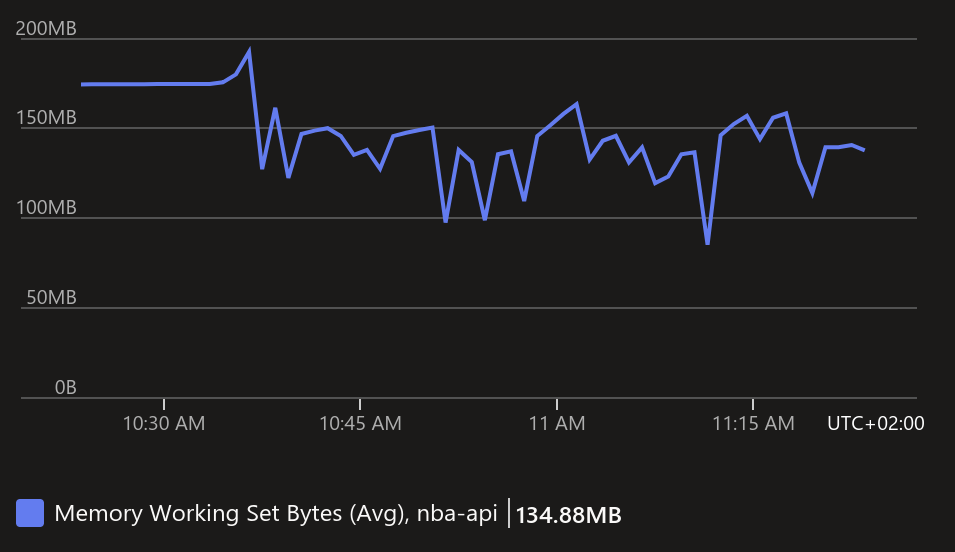
\includegraphics[width=0.5\textwidth]{img/load_test/nba-api-mem-avg.png} & 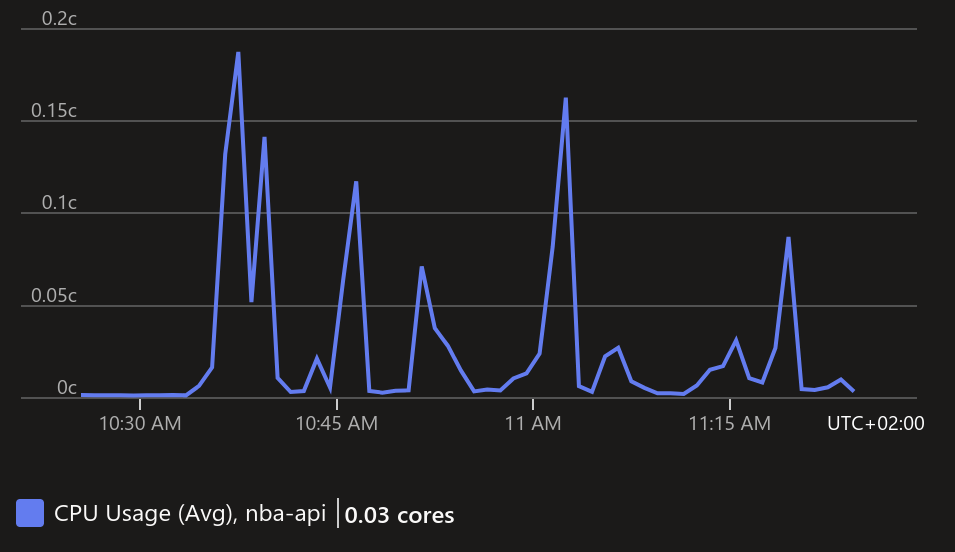
\includegraphics[width=0.5\textwidth]{img/load_test/nba-api-cpu-avg.png} \\
    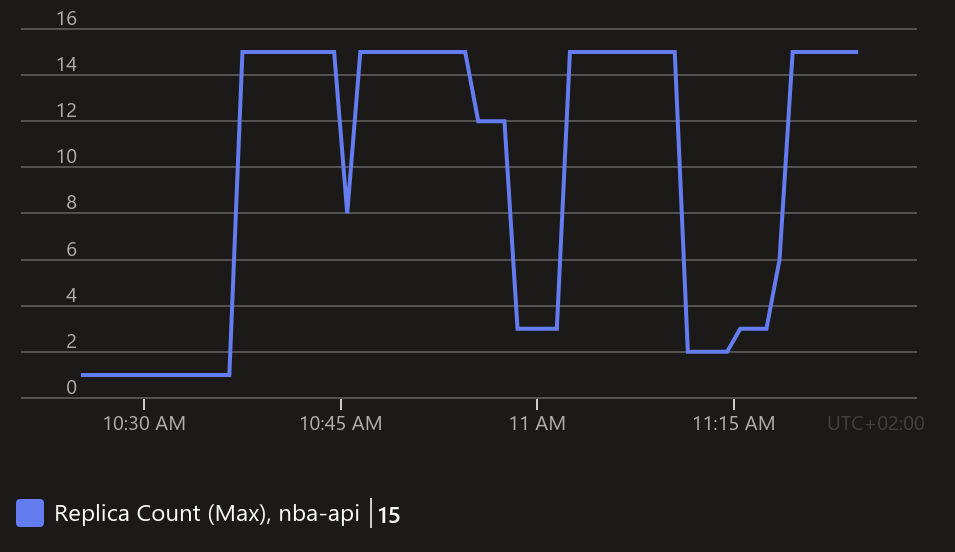
\includegraphics[width=0.5\textwidth]{img/load_test/nba-api-rep-count.png} & 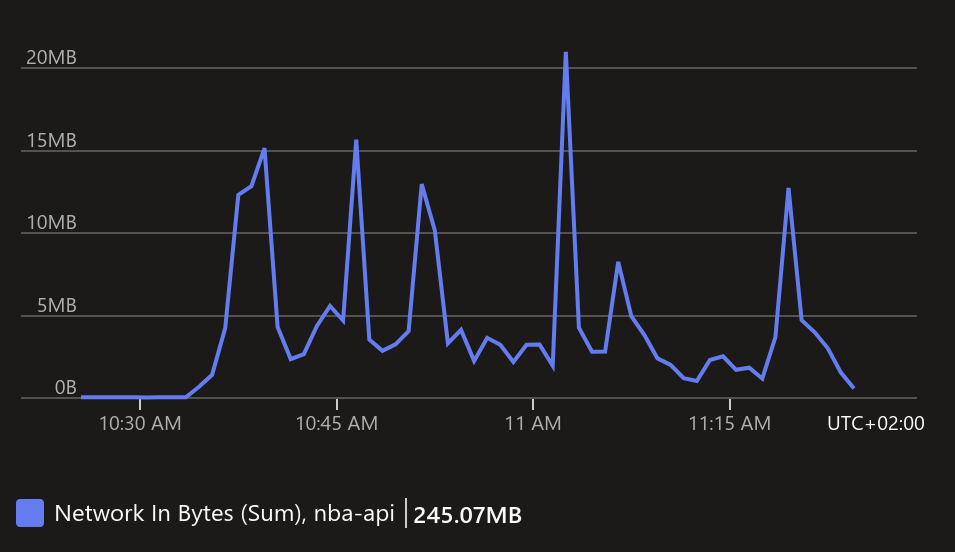
\includegraphics[width=0.5\textwidth]{img/load_test/nba-api-rx-sum.png} \\
\end{tabular}

Di seguito si riportano alcuni grafici che mostrano l'andamento di utilizzo delle risorse durante il test di Bet Api.

\begin{tabular}{ c c }
    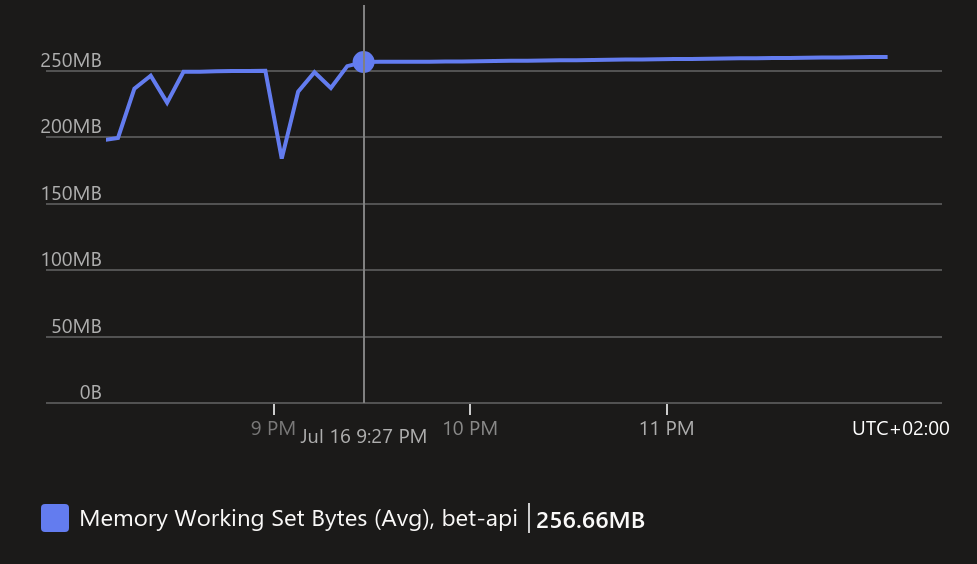
\includegraphics[width=0.5\textwidth]{img/load_test/bet-api-mem-avg.png} & 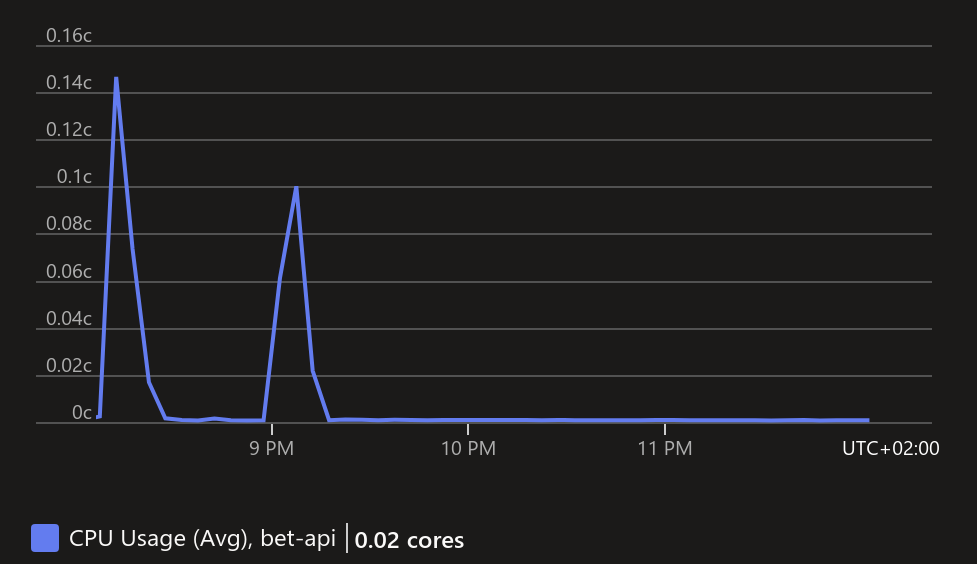
\includegraphics[width=0.5\textwidth]{img/load_test/bet-api-cpu-avg.png} \\
    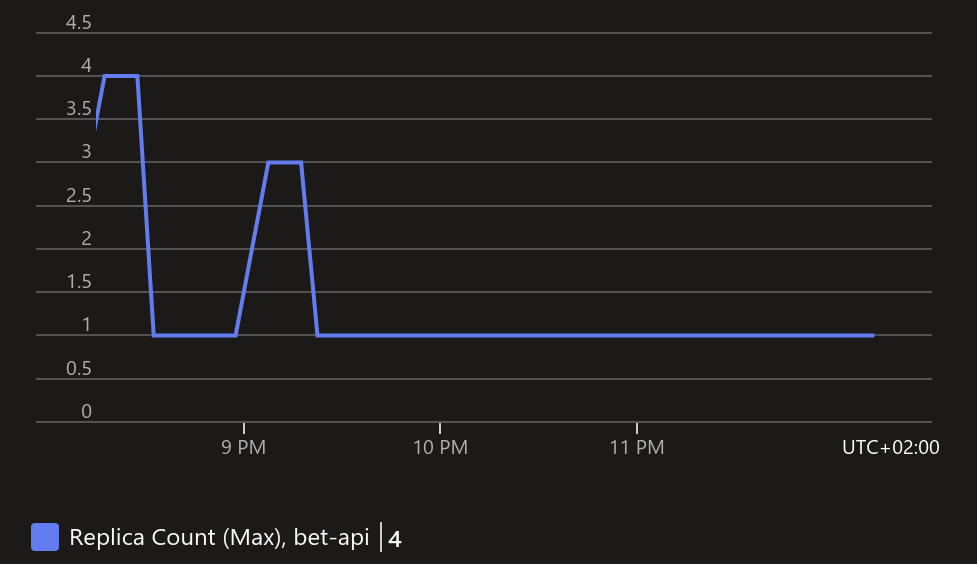
\includegraphics[width=0.5\textwidth]{img/load_test/bet-api-rep-count.png} & 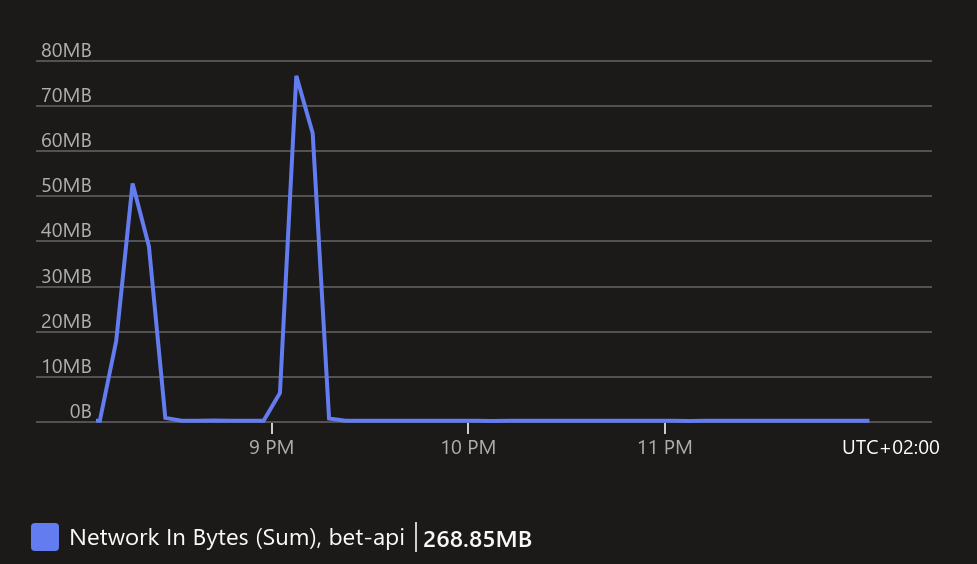
\includegraphics[width=0.5\textwidth]{img/load_test/bet-api-rx-sum.png} \\
\end{tabular}



\subsection{Stima costi}















